\documentclass[11pt, oneside]{article}   	% use "amsart" instead of "article" for AMSLaTeX format
\usepackage{geometry}                		% See geometry.pdf to learn the layout options. There are lots.
\geometry{letterpaper}                   		% ... or a4paper or a5paper or ... 
%\geometry{landscape}                		% Activate for rotated page geometry
%\usepackage[parfill]{parskip}    		% Activate to begin paragraphs with an empty line rather than an indent
\usepackage{graphicx}				% Use pdf, png, jpg, or eps§ with pdflatex; use eps in DVI mode
								% TeX will automatically convert eps --> pdf in pdflatex
\usepackage{amssymb}
\usepackage{amsmath}
\usepackage{algorithm}% http://ctan.org/pkg/algorithm
\usepackage{algpseudocode}% http://ctan.org/pkg/algorithmicx
%SetFonts

%SetFonts


\title{CSE512 HW1}
\author{Tim Zhang (110746199)}
\date{}							% Activate to display a given date or no date

\begin{document}
\maketitle
%\section{}
%\subsection{}

\section{Linear Algebra}
\subsection{Question 1}
\subsubsection{}
Let $A \in \Bbb R^{n \times n}$.  It will be shown that the eigenvalues of $A$ are the same as the eigenvalues of $A^T$.

Finding the eigenvalues of $A$ we solve:

\begin{gather*}
det(A - \lambda I) = 0 \text{ iff}\\
det((A - \lambda I)^T) = 0 \text{ iff}\\
det(A^T - \lambda I^T) = 0 \text{ iff}\\
det(A^T - \lambda I) = 0 \text{ iff}\\
det(A - \lambda I) = det(A^T - \lambda I) \text{ } \blacksquare
\end{gather*} 

\subsubsection{}
Let $M \in \Bbb R^{n \times n}$ such that $\lambda_i$ is the $ith$ eigenvalue of $M$ and let $x_i \in \Bbb R$ be the $ith$ eigenvector of $M$.  Then:

\begin{gather}
Mx_i = \lambda_i x_i \\
\alpha Mx_i = \alpha \lambda_ix_i\\
(\alpha M + \beta I)x_i = (\alpha \lambda_i + \beta)x_i
\end{gather}

Where $(3)$ follows since: 
\begin{gather*}
(\alpha M + \beta I)x_i = \alpha M x_i + \beta I x_i \\
= \alpha\lambda_i x_i + \beta x_i \\
= (\alpha\lambda_i + \beta)x_i
\end{gather*}

So the $ith$ eigenvalue of $\alpha M + \beta I$ is $\alpha \lambda_i + \beta$ $\blacksquare$

\section{Basic Statistics}
\subsection{Question 2: Probabilities}
The following lemma will be used in subsequent proofs.\\
\textbf{Lemma: $\Bbb P(A \setminus B) = \Bbb P(A) - \Bbb P(A \cap B)$}\\
\textbf{Proof:}
\begin{gather*}
\Bbb P((A \cap B) \cup (A \setminus B)) = \Bbb P(A \cap B) + \Bbb P(A \setminus B) \\
\Bbb P(A \setminus B) = \Bbb P((A \cap B) \cup (A \setminus B)) - \Bbb P(A \cap B) \\
\Bbb P(A \setminus B) = \Bbb P(A) - \Bbb P(A \cap B)
\end{gather*}

Where the first equality holds since $(A \cap B) \cup (A \setminus B) = \emptyset$ $\blacksquare$

\subsubsection{$\Bbb P(B \cap \overline{A}) = \Bbb P(B) - \Bbb P(A \cap B)$}
\begin{gather*}
 \Bbb P(B \cap \overline{A}) =  \Bbb P(\Omega \setminus (\overline{B \cap \overline{A}})) \\
=  \Bbb P(\Omega \setminus (\overline{B} \cup A)) \\
= \Bbb P((\Omega \setminus \overline{B}) \setminus A) \\
= \Bbb P(B \setminus A) \\
= \Bbb P(B) - \Bbb P(A \cap B) \text{ } \blacksquare
\end{gather*}

\subsubsection{$P(A \cup B) = \Bbb P(A) + \Bbb P(B) - \Bbb P(A \cap B)$}
\begin{gather*}
\Bbb P(A \cup B) = \Bbb P(A \cup (\overline{A} \cap B)) \\
= \Bbb P(A \cup (\overline{A} \cap ((A \cap B) \cup (\overline{A} \cap B)))) \\
= \Bbb P((A \cup \overline{A}) \cap (A \cup ((A \cap B) \cup (\overline{A} \cap B)))) \\
= \Bbb P(\Omega \cap (A \cup ((A \cap B) \cup (\overline{A} \cap B)))) \\
= \Bbb P(A \cup ((A \cap B) \cup (\overline{A} \cap B))) \\
= \Bbb P((A \cup (A \cap B)) \cup (\overline{A} \cap B)) \\
= \Bbb P(A \cup (\overline{A} \cap B))
\end{gather*}

Since $A \cap (\overline{A} \cap B) = \emptyset$ it follows that:
\begin{gather*}
\Bbb P(A \cup (\overline{A} \cap B)) = \Bbb P(A) + P(\overline{A} \cap B) \\
= \Bbb P(A) + \Bbb P(\Omega \setminus \overline{(\overline{A} \cap B)}) \\
= \Bbb P(A) + \Bbb P(\Omega \setminus (A \cup \overline{B}) \\
= \Bbb P(A) + \Bbb P((\Omega \setminus \overline{B}) \setminus A) \\
= \Bbb P(A) + \Bbb P(B \setminus A) \\
= \Bbb P(A) + \Bbb P(B) - \Bbb P(A \cap B) \text{ } \blacksquare
\end{gather*}

\subsubsection{If $A \subset B$ then $\Bbb P(A) \leq \Bbb P(B)$}
\begin{gather*}
\Bbb P(A) + \Bbb P(B) = \Bbb P(A \cap B) + \Bbb P(B) \\
= \Bbb P(\Omega \setminus \overline{(B \cap A)}) + \Bbb P(B) \\
= \Bbb P(\Omega \setminus (\overline{B} \cup \overline{A})) + \Bbb P(B) \\
= \Bbb P((\Omega \setminus \overline{B}) \setminus \overline{A}) + \Bbb P(B) \\
= \Bbb P(B \setminus \overline{A}) + \Bbb P(B) \\
= \Bbb P(B) + \Bbb P(B) - \Bbb P(B \cap \overline{A})\\
\leq \Bbb P(B) + \Bbb P(B)
\end{gather*}

Where the first equality follows since $A \subset B$ which implies that $A \cap B = A$.  The final inequality holds since $\Bbb P(B \cap \overline{A}) \neq \emptyset$ and $\Bbb P(B \cap \overline{A}) \geq 0$ by axiom.

Therefore subtracting $\Bbb P(B)$ from both sides of the inequality $\Bbb P(A) \leq \Bbb P(B)$ $\blacksquare$

\textbf{NOTE:} I believe that the stronger condition that $\Bbb P(A) < \Bbb P(B)$ actually holds since in the final inequality $\Bbb P(B \cap \overline{A}) = \emptyset$ only when $A = \Omega$, but $A \subset B$ and there is no such $B$ where $\Omega \subset B$ so $\Bbb P(B \cap \overline{A}) > 0$.  However the question stated to prove the weaker condition.

\newpage{}
\subsection{Question 3: Gaussian Distribution}
\subsubsection{$\Bbb E[X] = \mu$}
\begin{gather}
\Bbb E[X] = \int_{-\infty}^{\infty} xf(x)\\
= \int_{-\infty}^{\infty} x \frac{1}{\sigma\sqrt{2\pi}} \text{ } exp\bigg\{- \frac{(x - \mu)^2}{2\sigma^2}\bigg\} dx\\
=  \frac{1}{\sigma\sqrt{2\pi}} \int_{-\infty}^{\infty} (z + \mu) \text{ } exp\bigg\{- \frac{z^2}{2\sigma^2}\bigg\} dz\\
= \frac{1}{\sigma\sqrt{2\pi}} \bigg(\int_{-\infty}^{\infty} z \text{ } exp\bigg\{- \frac{z^2}{2\sigma^2}\bigg\} dz + \int_{-\infty}^{\infty} \mu \text{ } exp\bigg\{- \frac{z^2}{2\sigma^2}\bigg\} dz\bigg) \\
= \frac{1}{\sigma\sqrt{2\pi}} \int_{-\infty}^{\infty} exp\bigg\{- \frac{z^2}{2\sigma^2}\bigg\} zdz +  \frac{1}{\sigma\sqrt{2\pi}} \int_{-\infty}^{\infty} \mu \text{ } exp\bigg\{- \frac{z^2}{2\sigma^2}\bigg\} dz \\
= \frac{1}{\sigma\sqrt{2\pi}} \int_{-\infty}^{\infty} exp\bigg\{- \frac{z^2}{2\sigma^2}\bigg\} zdz + \mu \frac{1}{\sigma\sqrt{2\pi}} \int_{-\infty}^{\infty} exp\bigg\{- \frac{z^2}{2\sigma^2}\bigg\} dz \\
= \mu \bigg( \frac{1}{\sigma\sqrt{2\pi}} \int_{-\infty}^{\infty} exp\bigg\{- \frac{z^2}{2\sigma^2}\bigg\} dz \bigg) \\
= \mu
\end{gather}

Where $(10)$ follows since: 
\begin{gather*}
\frac{1}{\sigma\sqrt{2\pi}} \int_{-\infty}^{\infty} exp\bigg\{- \frac{z^2}{2\sigma^2}\bigg\} zdz = \frac{1}{\sigma\sqrt{2\pi}}\bigg[  \int_{-\infty}^{0} exp\bigg\{- \frac{z^2}{2\sigma^2}\bigg\} zdz +  \int_{0}^{\infty} exp\bigg\{- \frac{z^2}{2\sigma^2}\bigg\} zdz \bigg]\\
= \frac{1}{\sigma\sqrt{2\pi}} \bigg[ - \sigma^2 \bigg[ exp\bigg\{ - \frac{z^2}{2\sigma^2} \bigg\} \bigg]_{-\infty}^{0} + - \sigma^2 \bigg[ exp\bigg\{ - \frac{z^2}{2\sigma^2} \bigg\} \bigg]_{0}^{\infty} \bigg]\\
= \frac{1}{\sigma\sqrt{2\pi}} \bigg[ -\sigma^2 \text{ } exp\bigg\{ \frac{-1}{2\sigma^2} \bigg\} + \sigma^2 \text{ } exp\bigg\{ \frac{-1}{2\sigma^2} \bigg\} \bigg] = 0
\end{gather*}

Also $(11)$ follows because $$ \frac{1}{\sigma\sqrt{2\pi}} \int_{-\infty}^{\infty} exp\bigg\{- \frac{z^2}{2\sigma^2}\bigg\} dz =  \int_{-\infty}^{\infty}\frac{1}{\sigma\sqrt{2\pi}} \text{ } exp\bigg\{- \frac{(x - \mu)^2}{2\sigma^2}\bigg\} dx = 1$$

by the definition of a probability density function $\blacksquare$
\newpage{}
\subsubsection{$Var[X] = \sigma^2$}
\begin{gather*}
Var[X] = \Bbb E[(X - \Bbb E[X])^2]\\
= \Bbb E[(X - \mu)^2] \\
= \int_{-\infty}^{\infty}(x - \mu)^2f(x)dx\\
= \frac{1}{\sigma\sqrt{2\pi}} \int_{-\infty}^{\infty}(x - \mu)^2 \text{ } exp\bigg\{- \frac{(x - \mu)^2}{2\sigma^2}\bigg\} dx
\end{gather*}
Letting $z = (x - \mu)/\sigma$:
\begin{gather*}
\frac{1}{\sigma\sqrt{2\pi}} \int_{-\infty}^{\infty}\sigma^2 z^2 \text{ } exp\bigg\{- \frac{z^2}{2}\bigg\} \sigma dz\\
= \frac{\sigma^2}{\sqrt{2\pi}} \int_{-\infty}^{\infty}z^2 \text{ } exp\bigg\{- \frac{z^2}{2}\bigg\} dz\\
= \frac{\sigma^2}{\sqrt{2\pi}} \int_{-\infty}^{\infty}z (z \text{ } exp\bigg\{- \frac{z^2}{2}\bigg\}) dz
\end{gather*}
Integrating by parts:
\begin{gather*}
\frac{\sigma^2}{\sqrt{2\pi}} \bigg( \bigg[ -z \text{ }  exp\bigg\{- \frac{z^2}{2}\bigg\} \bigg]_{-\infty}^{\infty} + \int_{-\infty}^{\infty} exp\bigg\{- \frac{z^2}{2}\bigg\}dz \bigg)\\
= 0 + \frac{\sigma^2}{\sqrt{2\pi}} \int_{-\infty}^{\infty} exp\bigg\{- \frac{z^2}{2}\bigg\}dz\\
= \sigma^2 \int_{-\infty}^{\infty}\frac{1}{\sqrt{2\pi}} \text{ } exp\bigg\{- \frac{(x - \mu)^2}{2\sigma^2}\bigg\} \frac{1}{\sigma}dx\\
= \sigma^2 \int_{-\infty}^{\infty}\frac{1}{\sigma\sqrt{2\pi}} \text{ } exp\bigg\{- \frac{(x - \mu)^2}{2\sigma^2}\bigg\} dx\\
= \sigma^2 \text{ } \blacksquare
\end{gather*}

\newpage{}
\subsection{Question 4: Poisson Distribution}
\subsubsection{$\Bbb E[f(k; \lambda)]$}
\begin{gather*}
\Bbb E[f(k; \lambda)] = \sum_{k = 0}^{\infty} k f(k, \lambda)\\
= \sum_{k = 1}^{\infty} k \frac{\lambda^k e^{-\lambda}}{k!}\\
= e^{-\lambda} \sum_{k = 1}^{\infty} k \frac{\lambda^k}{k!}\\
= e^{-\lambda} \sum_{k = 1}^{\infty} \frac{\lambda^k}{(k - 1)!}\\
= \lambda e^{-\lambda} \sum_{k = 1}^{\infty} \frac{\lambda^{k - 1}}{(k - 1)!}\\
= \lambda e^{-\lambda} \sum_{z = 0}^{\infty} \frac{\lambda^{z}}{(z)!}\\
= \lambda e^{-\lambda} e^{\lambda}\\
= \lambda e^{-\lambda + \lambda}\\
= \lambda \text{ } \blacksquare
\end{gather*}

\subsubsection{$Var[f(k; \lambda)]$}
Since $Var[X] = \Bbb E[X^2] + \Bbb E[X]^2$ and $\Bbb E[X]^2$ is known to be $\lambda^2$ from the previous proof it suffices to compute $\Bbb E[X^2]$.
\begin{gather*}
\Bbb E[f(k^2; \lambda)] = \sum_{k = 0}^{\infty} k^2 f(k, \lambda)\\
= \sum_{k = 1}^{\infty} k^2 \frac{\lambda^k e^{-\lambda}}{k!}\\
= e^{-\lambda} \sum_{k = 1}^{\infty} k^2 \frac{\lambda^k}{k!}\\
= \lambda e^{-\lambda} \sum_{k = 1}^{\infty} k \frac{\lambda^{k - 1}}{(k - 1)!}\\
= \lambda e^{-\lambda} \bigg[ \sum_{k = 1}^{\infty} (k - 1) \frac{\lambda^{k - 1}}{(k - 1)!} + \sum_{k = 1}^{\infty} \frac{\lambda^{k - 1}}{(k - 1)!} \bigg]\\
= \lambda e^{-\lambda} \bigg[ \lambda \sum_{k = 2}^{\infty} \frac{\lambda^{k - 2}}{(k - 2)!} + e^\lambda \bigg]\\
= \lambda (\lambda e^{-\lambda} e^\lambda + e^{-\lambda} e^\lambda))\\
= \lambda(\lambda + 1)\\
= \lambda^2 + \lambda
\end{gather*}

Then using the definition of $Var[X]$:

\begin{gather*}
Var[f(k; \lambda)] = \lambda^2 + \lambda - \lambda^2\\
= \lambda \text{ } \blacksquare
\end{gather*}

\subsubsection{$Z = X_1 + X_2$ is Poisson distributed}
We want to show that $\Bbb P[Z = k] = \frac{\lambda^k e^{-\lambda}}{k!}$ for some $\lambda$.
\begin{gather*}
\Bbb P[Z = k] = \sum_{i = 0}^{k} \Bbb P[X_1 = i, X_2 = k - i]\\
= \sum_{i = 0}^{k} \Bbb P[X_1 = i] \times \Bbb P[X_2 = k - i]\\
= \sum_{i = 0}^{k} \frac{\lambda_1^i e^{-\lambda_1}}{i!} \times \frac{\lambda_2^{k - i} e^{-\lambda_2}}{(k - i)!}\\
= e^{-\lambda_1}e^{-\lambda_2} \sum_{i = 0}^{k} \frac{\lambda_1^i }{i!} \times \frac{\lambda_2^{k - i} }{(k - i)!}\\
= e^{- (\lambda_1 + \lambda_2)} \sum_{i = 0}^{k} \frac{\lambda_1^{i} \lambda_2^{k - i} }{i!(k - i)!}\\
= \frac{e^{- (\lambda_1 + \lambda_2)}}{k!} \sum_{i = 0}^{k} \frac{k!}{i!(k - i)!}\lambda_1^{i} \lambda_2^{k - i} \\
= \frac{e^{- (\lambda_1 + \lambda_2)}}{k!} \sum_{i = 0}^{k} {k \choose i}\lambda_1^{i} \lambda_2^{k - i} \\
= \frac{e^{- (\lambda_1 + \lambda_2)}}{k!} (\lambda_1 + \lambda_2)^k \\
\end{gather*}
Where the first equality holds since $Z = X_1 + X_2$ and the last equality holds due to the Binomial Theorem.  Then setting $\lambda = \lambda_1 + \lambda_2$ we have $\Bbb P[Z = k] = \frac{\lambda^k e^{-\lambda}}{k!}$ $\blacksquare$

\subsubsection{$\Bbb E[Z]$}
Since $Z$ is Poisson distributed $\Bbb E[Z] = \lambda = \lambda_1 + \lambda_2$.

\subsection{Question 5: Estimators}
\subsubsection{$\Bbb E[M_n] = \mu$}
Assuming that each $X_i$ has mean $\mu$:
\begin{gather*}
\Bbb E[M_n] = \Bbb E\bigg[\frac{1}{n} \sum_{i = 1}^{n} X_i\bigg] \\
= \frac{1}{n} \Bbb E\bigg[\sum_{i = 1}^{n} X_i\bigg] \\
= \frac{1}{n} \sum_{i = 1}^{n} \Bbb E[X_i] \\
= \frac{1}{n} \sum_{i = 1}^{n} \Bbb \mu \\
= \mu \text{ } \blacksquare
\end{gather*}

\subsubsection{$\Bbb E[S_n] = \sigma^2$}
Using the basic results from statistics that $Var[\overline{X}] = \frac{\sigma^2}{n}$ where $\overline{X} = \frac{1}{n}\sum_{i = 1}^{n}X_i = M_n$ and $Var[X] = \Bbb E[X^2] - \Bbb E[X]^2$:
\begin{gather*}
\Bbb E[S_n] = \Bbb E\bigg[\frac{1}{n - 1} \sum_{i = 1}^{n} (X_i - M_n)^2\bigg] \\
= \frac{1}{n - 1} \Bbb E\bigg[ \sum_{i = 1}^{n} X{_i}^2 - 2X_i M_n  + M{_n}^2 \bigg] \\
= \frac{1}{n - 1} \Bbb E\bigg[ \sum_{i = 1}^{n} X{_i}^2 - \sum_{i = 1}^{n} 2X_i M_n  + \sum_{i = 1}^{n} M{_n}^2 \bigg] \\
= \frac{1}{n - 1} \Bbb E\bigg[ \sum_{i = 1}^{n} X{_i}^2 - 2M_n \sum_{i = 1}^{n}  X_i  + \sum_{i = 1}^{n} M{_n}^2 \bigg] \\
= \frac{1}{n - 1} \Bbb E\bigg[ n X{_i}^2 - 2n M{_n}^2 + n M{_n}^2 \bigg] \\
= \frac{1}{n - 1} \Bbb E[ nX{_i}^2 - n M{_n}^2 ] \\
= \frac{1}{n - 1} \bigg[ n \Bbb E[ X{_i}^2 ] - n \Bbb E[ M{_n}^2 ] \bigg] \\
= \frac{1}{n - 1} \bigg[ n(Var[X] + \Bbb E[X]^2) - n(Var[M_n] + \Bbb E[M_n]^2) \bigg] \\
= \frac{1}{n - 1} \bigg[ n(\sigma^2 + \mu^2) - n(\frac{\sigma^2}{n} + \mu^2) \bigg] \\
= \frac{1}{n - 1} \bigg[ n\sigma^2 + n\mu^2 - \sigma^2 - n\mu^2) \bigg] \\
= \frac{1}{n - 1} (n - 1)\sigma^2 \\
= \sigma^2 \text{ } \blacksquare
\end{gather*}

\newpage{}
\subsubsection{Expectation Implementation}
Data samples are generated from a normal Gaussian distribution for both estimator implementations.

\begin{verbatim}
total = 0;              % Tracks total of current iteration
limit = 10000;          % Total number of iterations
means = zeros(limit);   % Array of means for plotting
count = (1:limit);      % Array of [1..limit] for plotting

for i = 1:limit
    for j = 1:i
        total = total + randn;
    end
    
    mean = total / i;
    means(i) = mean;
    total = 0;
end
\end{verbatim}

\newpage{}

\begin{figure}
  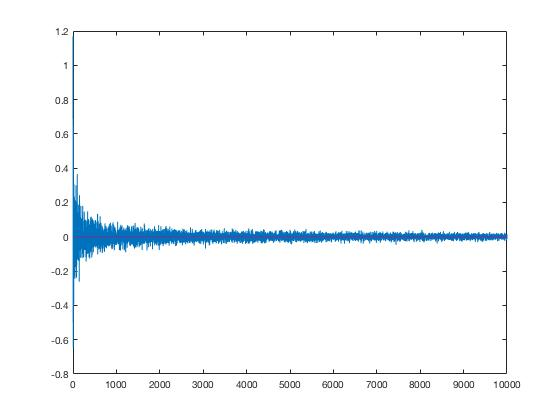
\includegraphics[width=\linewidth]{mean.jpg}
  \caption{Empirical mean with n=10000 iterations.}
\end{figure}

It looks as though the rate of convergence is around $O(n^{log(.5)})$.

\newpage{}
\subsubsection{Variance Implementation}
\begin{verbatim}
total = 0;                 % Tracks total of current iteration
limit = 10000;             % Total number of iterations
variances = zeros(limit);  % Array of means for plotting
count = (1:limit);         % Array of [1..limit] for plotting

for i = 1:limit
    samples = (1:i);  % Holds the samples for the current experiement
    
    % Generate each sample
    for j = 1:i
       samples(j) = randn;
    end
    
    % Calculate empirical mean of sample
    for j = 1:i
        total = total + samples(j);
    end
    
    mean = total / i;
    sum = 0;  % Total of the summation of variance
    
    % Calculate summation of variance
    for j = 1:i
        sum = sum + (samples(j) - mean)^2;
    end
    
    variance = (1 / (i - 1)) * sum;
    variances(i) = variance;
    total = 0;
end
\end{verbatim}

\newpage{}
\begin{figure}
  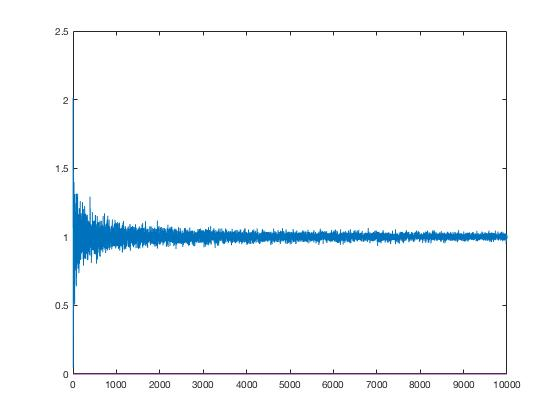
\includegraphics[width=\linewidth]{variance.jpg}
  \caption{Empirical variance with n=10000 iterations.}
\end{figure}

It looks as though the rate of convergence is around $O(n^{log(.55)})$.

\newpage{}
\section{(Agnostic) PAC Learning}

\subsection{Question 6}
\subsubsection{$\Bbb E[L_S(h_S)] \leq L_{\mathcal{D}}(h^*) \leq \Bbb E[L_{\mathcal{D}}(h_S)]$}
$\textbf{(1.)}$ $\Bbb E[L_S(h_S)] \leq L_{\mathcal{D}}(h^*)$

By definition $L_S(h_s)$ is minimized.  In the worst case $L_S(h_s) = L_{\mathcal{D}}(h^*)$, but otherwise $L_S(h_s) < L_{\mathcal{D}}(h^*)$.  Since in the worst case sampling the minimizer of $L_S$ is $h^*$ given that $h^*$ minimizes $L_{\mathcal{D}}$.  That is, there can only be better in-sample minimizers than $h^*$ but there are no worse ones. Which implies that in expectation $\Bbb E[L_S(h_S)] \leq L_{\mathcal{D}}(h^*)$.\\ \\
$\textbf{(2.)}$ $L_{\mathcal{D}}(h^*) \leq \Bbb E[L_{\mathcal{D}}(h_S)]$

By definition $L_{\mathcal{D}}(h^*)$ is minimized.  So $\forall h_S$, $L_{\mathcal{D}}(h_S) \geq L_{\mathcal{D}}(h^*)$.  This implies that in expectation $L_{\mathcal{D}}(h^*) \leq \Bbb E[L_{\mathcal{D}}(h_S)]$ by a similar argument as in \textbf{(1.)} $\blacksquare$

\subsubsection{Explanation}
The inequality essentially states that the difference between our in sample error and out of sample error is bounded by a function which depends on the confidence of our assertion ($\delta$) and the number of samples which we have collected.  In practice, if we were to collect a large number of samples we would see our out of sample error become a small value with high probability.  The number of samples needed is directly related to the confidence level we choose of course.

\subsection{Question 7}
\subsubsection{If $\mathcal{F}$ is agnostic PAC learnable then $\mathcal{F}$ is PAC learnable}
Let $\mathcal{F}$ be a hypothesis class of binary classifiers such that $\mathcal{F}$ is agnostic PAC learnable.  Then $\forall \epsilon, \delta \in (0, 1)$ and every distribution $\mathcal{D}$ over $\mathcal{X} \times \mathcal{Y}$, when running the learning algorithm on $m > m_{\mathcal{F}}$ i.i.d. examples generated by $\mathcal{D}$ and returning a hypothesis $h$ we have that with probability of at least $(1 - \delta)$ that $L_{\mathcal{D}}(h) \leq \min_{h' \in \mathcal{F}} L_{\mathcal{D}}(h') + \epsilon$.

By definition of PAC learnability, consider all distributions $\mathcal{D}$ with respect to $\mathcal{F}$ such that the realizability assumption holds.  Then $\exists h^* \in \mathcal{F}$ such that $L_{\mathcal{D}}(h^*) = 0$.  Which implies that: 
\begin{gather*}
L_{\mathcal{D}}(h) \leq \min_{h' \in \mathcal{F}} L_{\mathcal{D}}(h') + \epsilon\\
 = L_{\mathcal{D}}(h^*) + \epsilon\\ 
= \epsilon. 
\end{gather*}

So $\mathcal{F}$ is PAC learnable $\blacksquare$

\subsubsection{If $A$ is a successful agnostic PAC learner for $\mathcal{F}$ then $A$ is a successful PAC learner for $\mathcal{F}$}
Let $A$ be a successful agnostic PAC learner for $\mathcal{F}$.  Then for all samples $S$ generated from $\mathcal{D}$, $A(S) = h_S$ and $L_{\mathcal{D}}(h_S) \leq \min_{h' \in \mathcal{F}} L_{\mathcal{D}}(h') + \epsilon$.

Assume that $\mathcal{F}$ is realizable, then $L_{\mathcal{D}}(h_S) \leq \epsilon$ by the same argument above.  Thus $A$ is also a successful PAC learner for $\mathcal{F}$ $\blacksquare$
\newpage{}
\section{Least Square Regression}
\subsection{Question 8}
\subsubsection{train\_ls.m}
\begin{verbatim}
function [w, w_0] = train_ls(X, y, bias)
    dim = size(X);
    
    % Add a row of all 1's for bias term
    if bias
        inX = zeros(dim(1), dim(2) + 1);
        for i = 1:dim(1)
            inX(i, :) = [1 X(i, :)];
        end
    else
        inX = X;
    end
    
    % Check for invertibility
    if det(inX.' * inX) == 0
        [V, D] = eig(inX.' * inX);
        D_plus = zeros(size(D));
        
        % Create the positive D matrix as discussed in lecture slides
        for i = 1:(size(D))(1)
            for j = 1:(size(D))(2)
                if D(i, j) ~= 0
                    D_plus(i, j) = 1/D(i, j);
                end
            end
        end
        
        w = V * D_plus * V.' * inX.' * y;
        
    % Otherwise return the normal solution
    else
        w = inv(inX.' * inX) * inX.' * y;
    end
    
    % If a bias term is used in X then we need to move the value
    % from w to w_0
    if bias
        w_0 = w(1);
        w = w(2:length(w));
    else
        w_0 = 0;
    end 
end
\end{verbatim}

\newpage{}
\subsubsection{incremental\_train\_ls.m}
\begin{verbatim}
function w = incremental_train_ls(X, y)
    [m, d] = size(X);     % Dimensions of data
    inc_X = zeros(m, d);  % Used to ensure that inc_X is invertible
    w = zeros(1, d);      % Weights to be learned
    
    % Ensures that inc_X is invertible
    inc_X(1:d, 1:d) = 10^-4 * eye(d);
    
    % Calculate the first weights
    inc_X(1, :) = X(1, :);
    sm_inv = inv(inc_X.' * inc_X);  % Hold the inverse
    w = sm_inv * inc_X.' * y;
    
    if m > 1
        % Incrementally update the weights
        for i = 2:m
            next = X(i, :);  % The next training example
            inc_X(i, :) = next;  % Add next into X
            next = next.';  % Convert into column vector
            
            % Compute SM inverse
            top = sm_inv * (next * next.') * sm_inv;
            bottom = 1 + (next.' * sm_inv * next);
            sm_inv = sm_inv - (top / bottom);
            
            % Compute OLS optimization
            w = sm_inv * inc_X.' * y;
        end
    end
end
\end{verbatim}

\newpage{}
\subsubsection{Verification}
Shown below is a randomly generated sample which shows the numerical equivalence of the two procedures where $X \in \Bbb R^{100 \times 7}$ and $y \in \Bbb R^{100 \times 1}$
\begin{verbatim}
>> X = rand(100, 7)

X =

    0.1538    0.8241    0.6389    0.8099    0.5949    0.4613    0.8278
    0.9618    0.2182    0.7027    0.6378    0.5351    0.1100    0.6032
    0.8763    0.0996    0.8609    0.8981    0.3336    0.7813    0.8178
    0.4886    0.6195    0.3797    0.6218    0.8547    0.4534    0.9555
    0.4071    0.1038    0.7121    0.4146    0.2656    0.2971    0.6504
    0.1266    0.7991    0.5235    0.6476    0.9339    0.3584    0.6276
    0.9254    0.9029    0.3635    0.4893    0.3898    0.4824    0.6466
    0.0056    0.3125    0.4347    0.0938    0.6831    0.4312    0.0621
    0.1864    0.2816    0.6876    0.6373    0.2750    0.6988    0.9382
    0.3241    0.0068    0.2269    0.9503    0.0280    0.6751    0.8987
    0.0502    0.4959    0.9790    0.4764    0.9406    0.0069    0.6949
    0.1445    0.9885    0.9757    0.6028    0.5340    0.0790    0.3104
    0.7294    0.7379    0.2895    0.5915    0.6712    0.4606    0.3435
    0.4823    0.3107    0.3384    0.2253    0.6075    0.7775    0.0762
    0.3381    0.6004    0.9964    0.6684    0.7509    0.8168    0.5198
    0.2368    0.7817    0.7890    0.1566    0.9813    0.6314    0.6088
    0.4509    0.1115    0.7949    0.7743    0.7277    0.3649    0.7272
    0.1855    0.5793    0.6324    0.2131    0.8573    0.8875    0.0001
    0.3243    0.8704    0.8115    0.1691    0.9918    0.2509    0.1698
    0.2640    0.6898    0.4481    0.7258    0.7595    0.0661    0.4633
    0.8301    0.2430    0.8306    0.2562    0.1460    0.7272    0.3619
    0.6964    0.3427    0.1267    0.1628    0.3263    0.7668    0.9521
    0.3335    0.5454    0.5133    0.6258    0.0288    0.8983    0.9322
    0.5802    0.0676    0.7159    0.2507    0.6946    0.7668    0.9581
    0.2878    0.4104    0.2481    0.2630    0.9588    0.9469    0.2065
    0.2640    0.2375    0.5319    0.8439    0.7290    0.5357    0.1597
    0.2599    0.4890    0.3822    0.3974    0.7368    0.9598    0.5718
    0.6771    0.8061    0.8018    0.1046    0.1746    0.9782    0.5929
    0.5198    0.3778    0.6709    0.1939    0.3554    0.5221    0.6986
    0.0768    0.5180    0.9829    0.3631    0.5746    0.8454    0.3058
    0.0558    0.0946    0.9368    0.8745    0.4599    0.8980    0.3939
    0.2587    0.9091    0.5763    0.5998    0.8337    0.9312    0.3369
    0.4399    0.2076    0.0802    0.2581    0.8154    0.4576    0.1290
    0.2843    0.3821    0.4138    0.3584    0.3240    0.7592    0.0869
    0.6788    0.6603    0.1808    0.8875    0.4617    0.9388    0.5489
    0.9496    0.7584    0.9956    0.9005    0.6740    0.8107    0.3177
    0.7740    0.1731    0.5204    0.4480    0.5952    0.9304    0.9927
    0.6361    0.5174    0.8853    0.2689    0.1344    0.4470    0.7236
    0.7536    0.9953    0.6483    0.5538    0.0195    0.8339    0.5721
    0.7468    0.7076    0.4663    0.1788    0.1251    0.9878    0.7172
    0.5860    0.0806    0.0953    0.8597    0.2233    0.3696    0.9766
    0.7731    0.0433    0.9678    0.2320    0.4491    0.1708    0.4270
    0.3925    0.4912    0.6201    0.1681    0.5345    0.8232    0.9130
    0.6053    0.4466    0.1560    0.0267    0.9904    0.5871    0.8973
    0.2474    0.4868    0.3984    0.3224    0.7173    0.9616    0.8352
    0.2902    0.1659    0.8825    0.5552    0.9801    0.4891    0.0480
    0.0193    0.3607    0.5390    0.8245    0.0537    0.2535    0.3593
    0.3473    0.8807    0.5437    0.8042    0.6369    0.6782    0.2958
    0.1418    0.7444    0.4425    0.0244    0.9604    0.9145    0.6291
    0.4115    0.4168    0.1837    0.3715    0.2699    0.6171    0.1362
    0.1531    0.9074    0.2492    0.4919    0.9494    0.3225    0.3740
    0.8290    0.0943    0.2851    0.4661    0.9022    0.4905    0.8648
    0.7392    0.1813    0.5295    0.0417    0.1946    0.4075    0.2503
    0.0989    0.9466    0.5598    0.6170    0.7340    0.0839    0.0295
    0.8206    0.1008    0.4151    0.5780    0.1749    0.5920    0.9994
    0.2271    0.3880    0.9057    0.2988    0.1051    0.8790    0.6051
    0.1069    0.2892    0.3051    0.4357    0.3141    0.5533    0.2442
    0.6628    0.0731    0.6498    0.1366    0.3488    0.2995    0.4382
    0.9546    0.1946    0.2888    0.2997    0.3990    0.8970    0.7351
    0.8146    0.4175    0.2553    0.7614    0.2839    0.7943    0.5580
    0.6233    0.2929    0.3582    0.0353    0.3139    0.7758    0.4383
    0.3283    0.7021    0.8059    0.2695    0.7183    0.5990    0.6035
    0.2774    0.2397    0.5389    0.9963    0.9446    0.5572    0.1810
    0.4344    0.9595    0.5901    0.4469    0.0878    0.2997    0.8088
    0.3503    0.3055    0.2311    0.1528    0.2795    0.5477    0.8191
    0.8778    0.1549    0.1019    0.8862    0.5962    0.9918    0.4872
    0.0062    0.5555    0.6446    0.0314    0.8284    0.4834    0.7551
    0.6964    0.7905    0.9801    0.1160    0.7822    0.6848    0.4044
    0.3381    0.4439    0.1017    0.2509    0.5572    0.4800    0.7257
    0.3050    0.9958    0.1879    0.7597    0.0363    0.7465    0.1540
    0.6481    0.4366    0.0094    0.8983    0.6694    0.2114    0.5091
    0.9211    0.3044    0.8383    0.2234    0.8490    0.2485    0.6680
    0.8931    0.2465    0.4813    0.6733    0.0655    0.0978    0.1526
    0.9972    0.9608    0.4685    0.8188    0.3608    0.7087    0.0627
    0.0729    0.2229    0.9085    0.9489    0.2581    0.8557    0.3371
    0.1296    0.3956    0.4171    0.8743    0.4326    0.7890    0.4459
    0.9816    0.2245    0.5441    0.3937    0.3061    0.7428    0.7576
    0.0902    0.2700    0.6990    0.9370    0.9666    0.1045    0.1305
    0.6862    0.4184    0.0791    0.4369    0.1299    0.5209    0.9015
    0.9290    0.9977    0.5094    0.1625    0.2174    0.8466    0.2203
    0.1418    0.9110    0.4869    0.3098    0.8934    0.8436    0.3786
    0.8844    0.5504    0.8559    0.6811    0.6217    0.3777    0.4228
    0.0198    0.5963    0.6144    0.9341    0.3982    0.2721    0.9727
    0.3427    0.0791    0.1174    0.9474    0.3561    0.1253    0.1770
    0.2383    0.5766    0.6069    0.5991    0.6466    0.6914    0.8823
    0.9846    0.8982    0.1642    0.9489    0.7331    0.5551    0.5513
    0.8466    0.4633    0.3990    0.4040    0.7317    0.0085    0.3215
    0.7945    0.3984    0.5324    0.0410    0.9582    0.4160    0.8998
    0.9003    0.1045    0.8752    0.2938    0.0460    0.4391    0.5421
    0.7801    0.6522    0.6590    0.0319    0.4244    0.7844    0.4629
    0.8365    0.9917    0.7876    0.8645    0.0090    0.8300    0.8080
    0.3211    0.6781    0.1260    0.4325    0.7038    0.5896    0.3608
    0.7427    0.4285    0.5250    0.0928    0.7809    0.1421    0.9710
    0.6645    0.6548    0.8995    0.1378    0.5648    0.5933    0.5555
    0.2892    0.5887    0.1091    0.2420    0.0233    0.7262    0.7698
    0.3374    0.7451    0.6346    0.2230    0.0076    0.4284    0.6801
    0.9086    0.6409    0.0808    0.8677    0.9890    0.2108    0.2052
    0.0323    0.5037    0.4112    0.7642    0.2016    0.2654    0.8346
    0.6964    0.9380    0.7126    0.3447    0.8233    0.9932    0.8655
    0.2088    0.6053    0.1004    0.3848    0.3610    0.4808    0.0415

>> y = rand(100, 1)

y =

    0.6142
    0.2733
    0.7467
    0.4879
    0.7924
    0.5245
    0.5975
    0.2200
    0.3640
    0.2972
    0.8516
    0.9737
    0.6236
    0.8923
    0.9809
    0.6470
    0.7988
    0.4049
    0.4824
    0.0639
    0.8029
    0.3511
    0.8493
    0.9918
    0.4843
    0.3564
    0.0544
    0.9141
    0.7050
    0.4381
    0.9681
    0.7238
    0.6568
    0.5148
    0.8771
    0.0602
    0.4715
    0.3110
    0.1947
    0.1510
    0.9014
    0.0707
    0.9584
    0.6999
    0.0120
    0.0049
    0.8533
    0.4673
    0.8367
    0.2206
    0.8060
    0.2486
    0.9983
    0.9379
    0.5540
    0.9127
    0.6355
    0.7801
    0.5672
    0.1918
    0.9062
    0.5149
    0.9990
    0.3773
    0.2061
    0.7299
    0.3134
    0.1176
    0.8886
    0.6931
    0.9399
    0.4172
    0.8158
    0.8048
    0.3604
    0.9138
    0.2883
    0.1650
    0.4559
    0.2428
    0.0019
    0.6153
    0.6612
    0.6603
    0.6805
    0.8506
    0.0373
    0.6808
    0.5711
    0.6902
    0.8956
    0.2669
    0.0686
    0.3136
    0.7892
    0.4983
    0.4370
    0.1684
    0.2646
    0.6839

>> w = incremental(X, y)

w =

    0.0650
    0.0810
    0.1428
    0.3139
    0.0589
    0.2234
    0.1414

>> w = leastSquares(X, y, false)

w =

    0.0650
    0.0810
    0.1428
    0.3139
    0.0589
    0.2234
    0.1414
\end{verbatim}
$\blacksquare$

\newpage{}
\subsubsection{Analysis}
Assuming that matrix inversion takes $O(n^3)$, time the first algorithm computes on the full $m \times d$ input matrix while the second implementation only computes the full inversion on the first $x_i \in \Bbb R^{1 \times d}$. After the first inversion the incremental implementation spends the majority of it's time computing small matrix multiplications.  So it seems that if $m$ is relatively small then it would not hurt to use the numerical solution presented by OLS.  If on the other hand $m$ is large then the incremental approach would save computational time.
\newpage{}
\subsection{Question 9}
\subsubsection{Implementation}
\begin{verbatim}
%
% Driver function for polynomial linear regression
%
function polynomial(X_train, X_test, Y_train, Y_test, k)
    % Generate polynomial features
    poly_train = generate_poly_features(X_train, k);
    poly_test = generate_poly_features(X_test, k);
    
    % Normalize data
    [norm_poly_train, norm_poly_test] = normalizeAll(poly_train, poly_test);
    
    % Train using least squares
    [w, w_0] = train_ls(norm_poly_train, norm_Y_train, true);
    
    % Calculate the in sample errors
    trainLoss = squareError(w, w_0, norm_poly_train, norm_Y_train);
    testLoss = squareError(w, w_0, norm_poly_test, norm_Y_test);
    
    % Output errors
    fprintf('Training Error: %d\n', trainLoss);
    fprintf('Test Error: %d\n', testLoss);
end

%
% Function nomalizes training and test sets
%
function [X_train_norm, X_test_norm] = normalizeAll(X_train, X_test)
    trainMax = max(X_train);              % Maximum of training data features
    trainMin = min(X_train);              % Minimum of training data features
    testMax = max(X_test);                % Maximum of test data features
    testMin = min(X_test);                % Minimum of test data features
    trainSize = size(X_train);            % Dimensions of training data
    testSize = size(X_test);              % Dimensions of test data
    X_train_norm = zeros(size(X_train));  % Normalized training set
    X_test_norm = zeros(size(X_test));    % Normalized test set
    
    % Normalize the training data
    for i = 1:trainSize(1)
        for j = 1:trainSize(2)
            X_train_norm(i, j) = normalize(X_train(i, j), trainMax(j), trainMin(j));
        end
    end
    
    % Normalize the test data
    for i = 1:testSize(1)
        for j = 1:testSize(2)
            X_test_norm(i, j) = normalize(X_test(i, j), testMax(j), testMin(j));
        end
    end
end

%
% Function normalizes a datapoint w.r.t. the max and min elements
%
function y = normalize(x, maximum, minimum)
    y = 2 * ((x - minimum)/(maximum - minimum)) - 1;
end

%
% Function generates poylnomial features to the degree k from input matrix
%
function [X_poly] = generate_poly_features(X, k)
    length = size(X);                        % Original dimensions of X
    pDimensions = length(2) * k;             % Number of polynomail dimensions
    X_poly = zeros(length(1), pDimensions);  % Polynomial feature matrix
    
    % For every sample
    for m = 1:length(1)
        % For each dimension
        for d = 1:length(2)
            power = 1;  % Current power
            
            % Expand the feature k times
            for i = ((d - 1) * k) + 1:((((d - 1) * k) + 1) + (k - 1))
                X_poly(m, i) = X(m, d)^power;
                power = power + 1;
            end
        end
    end
end

%
% Calculates sample error of X on y w.r.t. w and w0
%
function loss = squareError(w, w0, X, y)
    dimensions = size(X);  % Size of input matrix
    m = dimensions(1);     % Number of samples
    loss = 0;              % Value of loss
    
    % Sum over each training example
    for i = 1:m
        loss = loss + (y(i) - (w0 + dot(w, X(i,:))))^2;
    end
    
    loss = loss / m;
end
\end{verbatim}
\subsubsection{Error Graphs}
Graphs are plotted using the in sample risk over the squared loss function.

\begin{figure}
  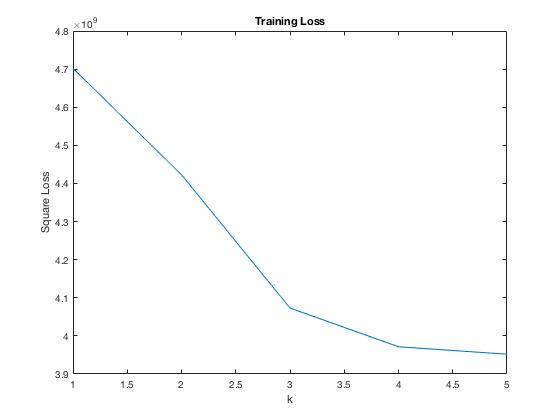
\includegraphics[width=\linewidth]{train-loss.jpg}
  \caption{Training loss over different values of k.}
\end{figure}

\begin{figure}
  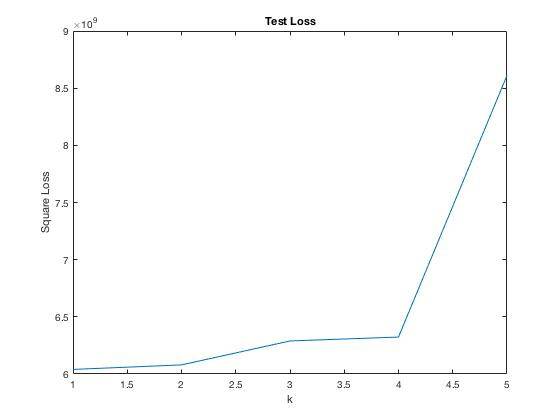
\includegraphics[width=\linewidth]{test-loss.jpg}
  \caption{Test loss over different values of k.}
\end{figure}

\subsubsection{Interpretation}
It is clear from the figures that as sample error decreases out of sample error increases.  I believe that this is because as we increase the value of $k$ we also increase the amount of overfitting that our function experiences with respect to the training data.  So, increasing the polynomial representation of the training data will lead to poor generalization with respect to out of sample examples.
\end{document} 